\documentclass[tikz,border=8pt]{standalone}
\usepackage{amsmath}
\usetikzlibrary{arrows.meta,positioning,fit}

\begin{document}
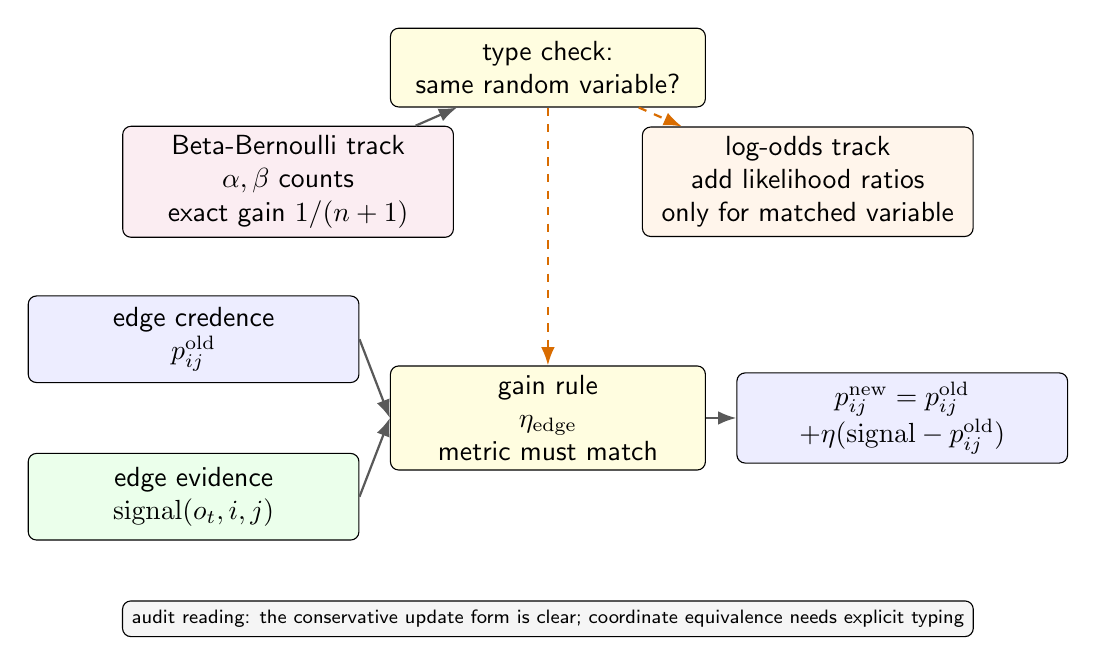
\begin{tikzpicture}[
  font=\sffamily,
  box/.style={draw, rounded corners=3pt, align=center, minimum width=42mm, minimum height=11mm, fill=white},
  gate/.style={draw, rounded corners=3pt, align=center, minimum width=40mm, minimum height=10mm, fill=yellow!12},
  note/.style={align=center, font=\sffamily\scriptsize},
  arrow/.style={-Latex, thick, draw=black!65},
  warn/.style={-Latex, thick, dashed, draw=orange!85!black}
]

\node[box, fill=blue!7] (old) at (0,0)
  {edge credence\\$p_{ij}^{\rm old}$};
\node[box, fill=green!8] (sig) at (0,-2)
  {edge evidence\\$\mathrm{signal}(o_t,i,j)$};
\node[gate] (gain) at (4.5,-1)
  {gain rule\\$\eta_{\rm edge}$\\metric must match};
\node[box, fill=blue!7] (newp) at (9,-1)
  {$p_{ij}^{\rm new}=p_{ij}^{\rm old}$\\$+\eta(\mathrm{signal}-p_{ij}^{\rm old})$};

\draw[arrow] (old.east) -- (gain.west);
\draw[arrow] (sig.east) -- (gain.west);
\draw[arrow] (gain.east) -- (newp.west);

\node[box, fill=purple!7] (beta) at (1.2,2.0)
  {Beta-Bernoulli track\\$\alpha,\beta$ counts\\exact gain $1/(n+1)$};
\node[box, fill=orange!8] (logodds) at (7.8,2.0)
  {log-odds track\\add likelihood ratios\\only for matched variable};
\node[gate] (type) at (4.5,3.45)
  {type check:\\same random variable?};

\draw[arrow] (beta) -- (type);
\draw[warn] (type) -- (logodds);
\draw[warn] (type.south) -- (gain.north);

\node[note, fill=gray!8, draw, rounded corners=3pt, minimum width=92mm] at (4.5,-3.55)
  {audit reading: the conservative update form is clear; coordinate equivalence needs explicit typing};

\end{tikzpicture}
\end{document}
